\documentclass[16pt]{beamer}
\usepackage{pgf}
\usepackage{beamerthemesplit}
\usepackage{url,graphicx,tabularx,array,geometry}
\setlength{\parskip}{1ex}
\setlength{\parindent}{0pt}
\usepackage{amssymb}
\usepackage{listings}
\usepackage{amsmath}
\usepackage{cite}
\usepackage{graphicx} 
\usepackage{animate}
\usepackage[utf8x]{inputenc}
\usepackage[english,italian]{babel}
\usepackage{hyperref}
\usepackage[italian]{babel}
\usepackage{amssymb}
%definizione colori template
\definecolor{BLU_TEMPLATE}{RGB}{100,0,0}


\usepackage{xcolor}
\usepackage[export]{adjustbox}

%utilizzo colori template
\setbeamercovered{transparent}
\mode<presentation>
\usetheme[numbers,totalnumber,compress,sidebarshades]{Berlin}
%\setbeamertemplate{footline}[frame number]

\usecolortheme[named=BLU_TEMPLATE]{structure}
\useinnertheme{circles}
\usefonttheme[onlymath]{serif}
\setbeamercovered{transparent}
\setbeamertemplate{blocks}[rounded][shadow=true]
\setbeamertemplate{navigation symbols}{}
\pgfdeclareimage[height=1.3cm]{university-logo}{unisa.jpg}
\logo{\pgfuseimage{university-logo}}


\title[A more efficient implementation of the subgraphs-world for the Glauber dynamics in the Ising model]{A more efficient implementation of the subgraphs-world for the Glauber dynamics in the Ising model}
\author[Francesco Farina]{Francesco Farina}
\institute[Laurea Magistrale in Informatica, Università degli Studi di Salerno]{Laurea Magistrale in Informatica\\Università degli Studi di Salerno}

\titlegraphic{
	%\ \ \ \  \ \  \ \
	\vspace{-12pt}
	{\bf Relatori} \hfill
	\ \ \\
	\small{Prof. Vincenzo Auletta} \hfill \ \ \\
	\small{Dott. Diodato Ferraioli}	\hfill  \ \ \\
	\vspace{-37pt}\hspace{260pt}
\includegraphics[scale=0.18]{images/logounisa.jpg}
}

\setbeamertemplate{itemize subitem}[triangle]

%inizio presentazione
\begin{document}


%titlepage e table of contents
\frame{\titlepage}
\begin{frame}{Overview}
	\tableofcontents[hideallsubsections]
\end{frame}


\section{Introduzione}

\frame{
	\frametitle{Tag Cloud}
	\begin{figure}
		\centering
		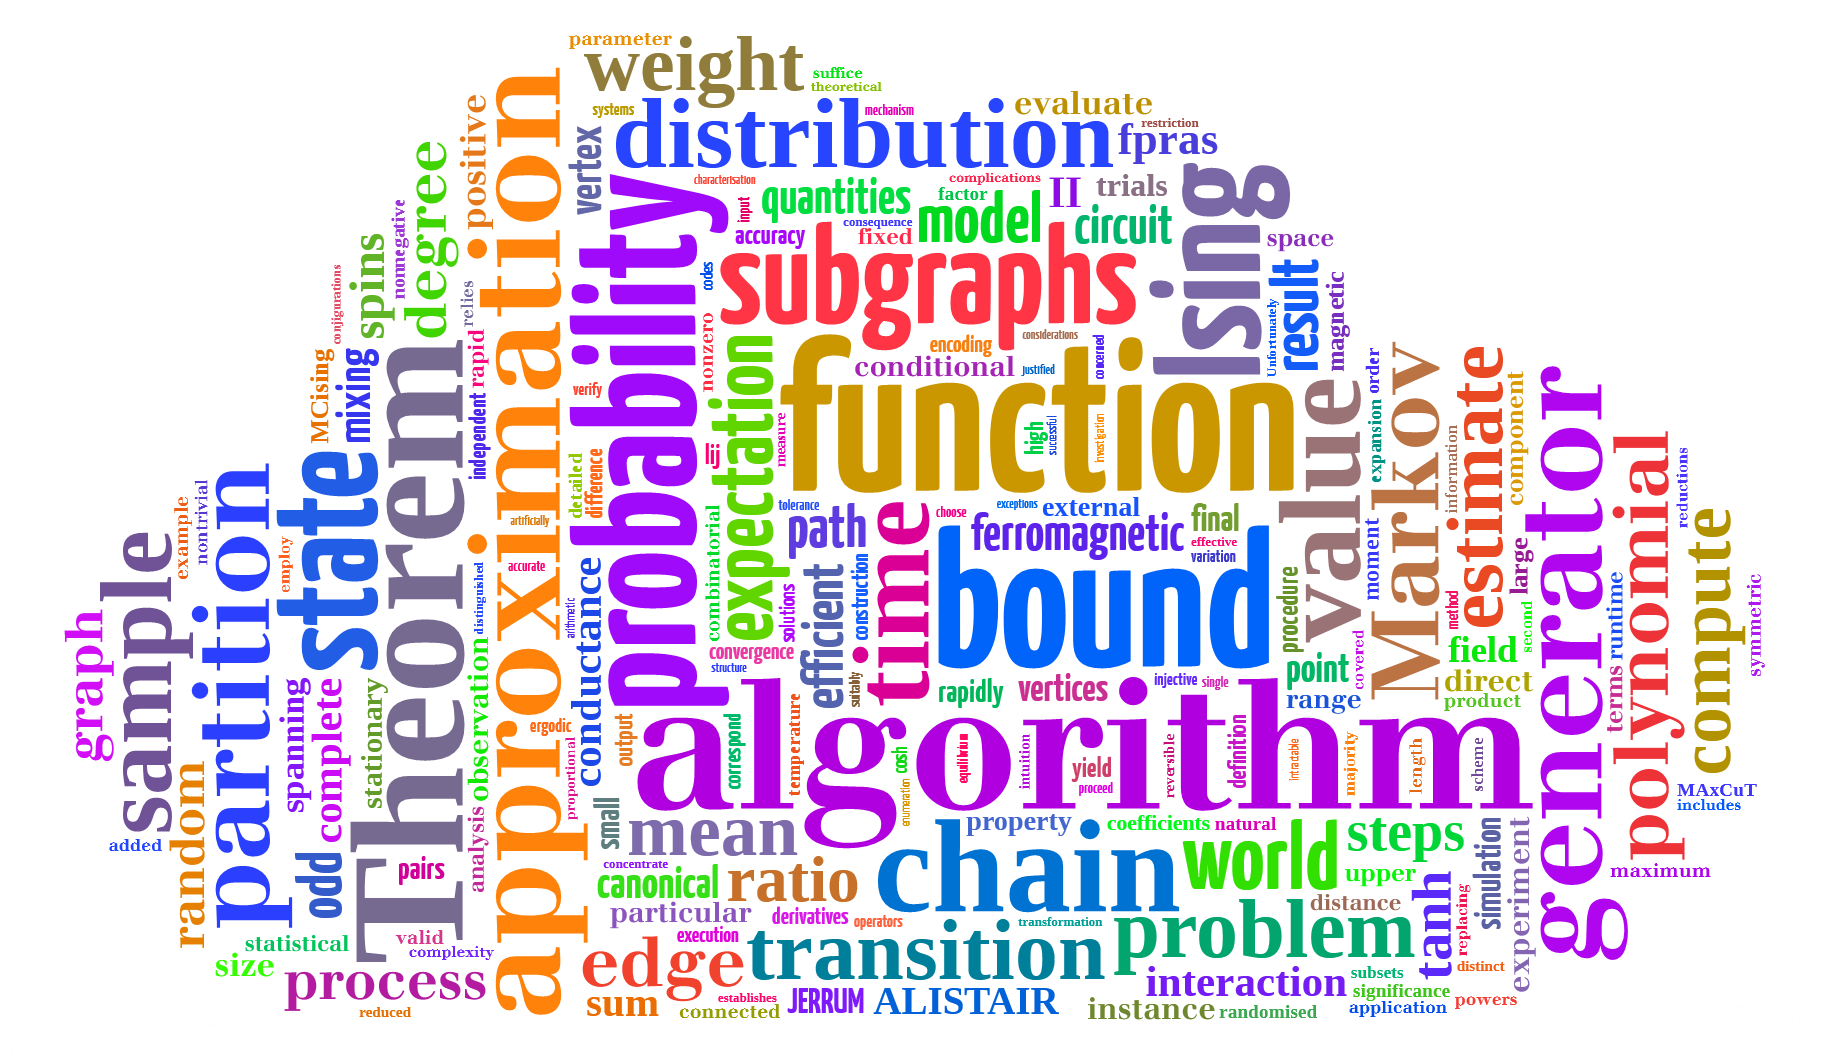
\includegraphics[scale=0.16]{img/cloud.png}
	\end{figure}
}


%Template
%\subsection{subsection}
%\frame{
%	\frametitle{titolo}
%	\begin{block}{}
%		asd \textbf{\color{BLU_TEMPLATE}asd} asd
%	\end{block}
%	\hfill\includegraphics[scale=0.15]{img/.png}
%}


\subsection{Concetti base}
\frame{
	\frametitle{Reti Sociali}
	\begin{block}{}
		La rapida crescita delle \textbf{\color{BLU_TEMPLATE}reti sociali} ha cambiato il modo in cui le persone interagiscono.
	\end{block}
	\pause
	\begin{block}{}
		Le informazioni si diffondono molto più velocemente.
	\end{block}
	\pause
	\begin{block}{}
		L'influenza di ogni singolo sui suoi vicini crea un'idea globale.
	\end{block}
	\hfill
\includegraphics[scale=0.3]{img/social-network2.png}
}

\frame{
	\frametitle{Sistema complesso}
	\begin{block}{}
		\begin{itemize}
			\item Insieme composto da più parti
			\begin{itemize}
				\item Ogni parte possiede uno o più obiettivi
			\end{itemize}
			\item Comportamento globale
			\begin{itemize}
				\item Determinato dall'interazione delle singole parti
			\end{itemize}
		\end{itemize}
	\end{block}
	\pause
	\begin{block}{}
		\begin{itemize}
			\item Rilevato in ambiti differenti
			\begin{itemize}
				\item Economico, fisico, informatico, biologico, ecc...
			\end{itemize}
			\item Fenomeni analoghi si verificano al loro interno
			\begin{itemize}
				\item Necessità di un linguaggio comune che modelli la struttura del sistema ed il comportamento delle parti
			\end{itemize}
		\end{itemize}
	\end{block}
	\hfill
\includegraphics[scale=0.15]{img/compl_sys.png}
}

\subsection{Linguaggi comuni}
\frame{
	\frametitle{Graph Theory}
	\begin{block}{}
		\begin{itemize}
			\item Descrive le relazioni che intercorrono tra oggetti di un insieme
			\begin{itemize}
				\item Branca della matematica nata nel 1700
			\end{itemize}
			\item \textit{Grafo}: struttura che descrive ed organizza tali relazioni
			\begin{itemize}
				\item \textit{Nodo}: oggetto dell'insieme
				\item \textit{Arco}: esprime la relazione tra coppie di oggetti
			\end{itemize}
		\end{itemize}
	\end{block}
	\hfill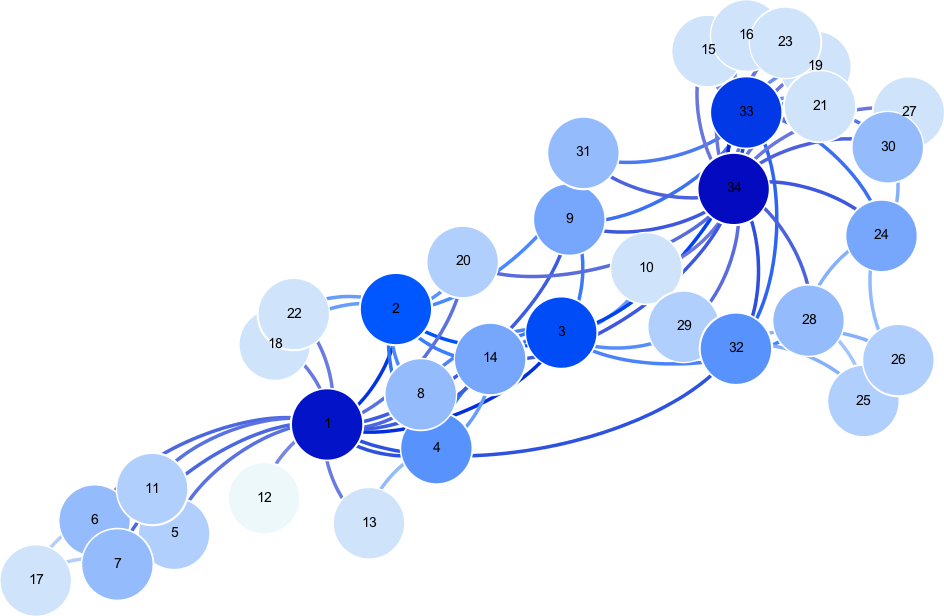
\includegraphics[scale=0.15]{img/zkc.png}
}

\frame{
	\frametitle{Game Theory}
	\begin{block}{}
		\begin{itemize}
			\item Modella il comportamento di agenti che devono prendere decisioni
			\begin{itemize}
				\item Situazioni di conflitto o interazione strategica
				\item Azioni che si influenzano a vicenda
			\end{itemize}
		\end{itemize}
	\end{block}
	\begin{block}{}
		\begin{itemize}
			\item Interazioni modellate come \textit{gioco}
			\begin{itemize}
				\item Giocatori
				\item Strategie
				\item Payoff
			\end{itemize}
		\end{itemize}
	\end{block}
	
	\vspace{-4pt}\hfill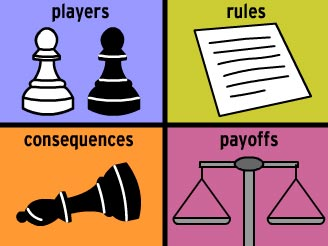
\includegraphics[scale=0.2, cfbox=BLU_TEMPLATE 1pt 1pt]{img/game-theory.jpg}
}

\frame{
	\frametitle{Game Theory classica}
	\begin{block}{}
		\begin{itemize}
			\item Giocatori pienamente razionali
			\begin{itemize}
				\item Conoscenza completa del gioco
				\item Potere computazionale illimitato
				\item Best response \textit{dynamics}
			\end{itemize}
			\item Non realistico nei casi del mondo reale
			\begin{itemize}
				\item Risorse limitate
			\end{itemize}
		\end{itemize}
	\end{block}
	\begin{block}{}
		\begin{itemize}
			\item Modellare la \textit{bounded rationality}
			\begin{itemize}
				\item Dinamica probabilistica
				\item Strategia giocata
				\begin{itemize}
					\item[--] \textit{Alta probabilità}: massima utilità
					\item[--] \textit{Bassa probabilità}: scelta sbagliata
				\end{itemize}
			\end{itemize}
		\end{itemize}
	\end{block}
}

\frame{
	\frametitle{Logit dynamics}
	\begin{block}{Definizione}
		\begin{itemize}
			\item Considera un gioco $\mathcal{G} = ([n], S_1,\ldots, S_n, u_1, \ldots, u_n)$
			\begin{itemize}
				\item $n$ giocatori
				\item $S_i$: insieme finito di strategie per il giocatore $i$
				\item $u_i$: funzione utilità per il giocatore $i$
			\end{itemize}
		\end{itemize}
	\end{block}
	\begin{block}{Ad ogni passo}
		\begin{itemize}
			\item Seleziona un giocatore $i$ a caso
			\item $i$ modifica la sua strategia in accordo alla \textit{logit update rule}
		\end{itemize}
	\end{block}
}

\frame{
	\frametitle{Logit update rule}
	\begin{block}{Strategia}
		$s \in S_i$ con probabilità $\sigma_i(s|x)=e^{\beta u_i(s,x_{-i})}/Z_i(x)$
	\end{block}
	\begin{block}{Parametri}
		\begin{itemize}
			\item $x$: corrente profilo di strategie
			\item $Z_i(x)$: fattore di normalizzazione
			\begin{itemize}
				\item $\sum_{z \in S_i}{e^{\beta u_i(s,x_{-i})}}$
			\end{itemize}
			\item $\beta$: grado di razionalità del sistema
			\begin{itemize}
				\item $\beta = 0$: scelta casuale
				\item $\beta > 0$: profili a payoff maggiore
				\item $\beta \rightarrow \infty$: \textit{best response}
			\end{itemize}
		\end{itemize}
	\end{block}
}

\frame{
	\frametitle{Logit dynamics}
	\begin{block}{Potential game}
		\begin{itemize}
			\item Se $\mathcal{G}$ è un potential game con funzione potenziale $\Phi$
			\begin{itemize}
				\item Distribuzione stazionaria $\rightarrow$ \textit{Gibbs measure}
				\begin{itemize}
					\item[--] $\pi(x) = \frac{1}{Z}e^{\beta\Phi(x)}$
				\end{itemize}
				\item Logit dynamics $\rightarrow$ \textit{Glauber dynamics}
				\item $Z \rightarrow$ \textit{Partition function}
				\begin{itemize}
					\item Descrive situazioni di equilibrio termodinamico
				\end{itemize}
			\end{itemize}
		\end{itemize}
	\end{block}
}

\subsection{\ }
\frame{
	\frametitle{Obiettivo del lavoro}
	\begin{block}{}
		Computare la {\color{BLU_TEMPLATE}\textit{Gibbs measure}}
	\end{block}
	\begin{block}{Applicazioni}
		\begin{itemize}
			\item Computare il \textit{Mean Magnetic Moment}
			\item Prevedere l'adozione di un prodotto da parte di una popolazione sotto campagna pubblicitaria
		\end{itemize}
	\end{block}
}

\frame{
	\frametitle{Obiettivo del lavoro (2)}
	\begin{block}{Approccio}
		\begin{itemize}
			\item Simulare la dinamica finché non raggiunge la distribuzione stazionaria
			\item \textbf{\color{BLU_TEMPLATE}Calcolare la \textit{partition function Z}}
			\begin{itemize}
				\item Problema \textit{{\small{\#}}P-hard}
				\begin{itemize}
					\item Limiti computazionali per ottenere \textit{Z}
				\end{itemize}
			\end{itemize}
		\end{itemize}
	\end{block}
	\begin{block}{Soluzione Approssimata}
		Catena di Markov alternativa
		\begin{itemize}
			\item Rapidly Mixing
			\item Distribuzione stazionaria da cui derivare quella di nostro interesse
		\end{itemize}
	\end{block}
}

%%%%%%%%%%%%%%%%%%%%%%%%%%%%%%%%%%%%%%%%%%%%%%%%%%%%%%%%%%%%%%%%%%%%%%%%%%%%

\section{Stato dell'arte}
\subsection{Lavori precedenti}
\frame{
	\frametitle{Modello fondamentale}
	\begin{block}{Polynomial-time approximation algorithms for the Ising model}
		\begin{itemize}
			\item Mark Jerrum ed Alistair Sinclair, 1993
			\item Algoritmo JS
			\begin{itemize}
				\item \textit{fully polynomial randomized approximation scheme} (fpras)
				\item Calcolo della \textbf{\color{BLU_TEMPLATE}partition function Z} della \textit{Gibbs measure}
				\item Descritto analiticamente
			\end{itemize}
		\end{itemize}
	\end{block}
}

\frame{
	\frametitle{Modello di Ising}
	\begin{block}{Configurazioni \textit{n} giocatori}
		\begin{itemize}
			\item Giocatore \textit{i}: $\sigma_i = \pm1$
			\item Configurazione $\sigma = (\sigma_1, \ldots, \sigma_n)$
			\item Peso archi
			\begin{itemize}
				\item $\forall(i,j) \in E : V_{ij}\neq0$
			\end{itemize} 
		\end{itemize}
	\end{block}
	\hfill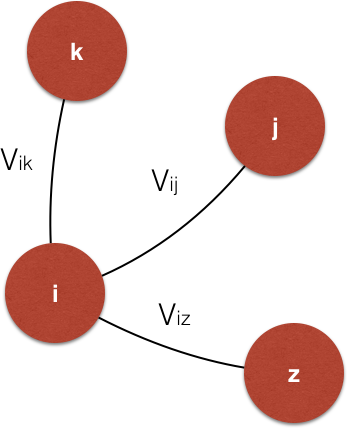
\includegraphics[scale=0.2]{img/ising.png}
}

\frame{
	\frametitle{Simulare la catena di Markov}
	\begin{block}{\textit{Spin-world process}}
		\begin{itemize}
			\item Stati: $2^n$ configurazioni del gioco
			\item Transizioni tra configurazioni che differiscono in una sola componente
			\item Non è \textit{rapidly mixing}
		\end{itemize}
	\end{block}
	\pause
	\begin{block}{\textit{Subgraphs-world process}}
		\begin{itemize}
			\item Processo generico
			\item Applicabile al modello di Ising
			\item È \textbf{\color{BLU_TEMPLATE}rapidly mixing}
		\end{itemize}
	\end{block}
}
\subsection{Soluzione J\&S}
\frame{
	\frametitle{Subgraphs-world process}
	\begin{block}{Configurazioni}
		\begin{itemize}
			\item \textit{Spanning subgraph} del grafo d'interazione del gioco $(n, E)$
			\item Sottografo che contiene tutti i nodi del grafo iniziale
			\item Configurazione $X$: peso $w(X)$
		\end{itemize}
	\end{block}
	\begin{block}{Catena di Markov ergodica}
		\begin{itemize}
			\item Stati: $2^m$ configurazioni, $m = |E|$
			\item Transizioni tra configurazioni che differiscono di un solo arco
			\item Distribuzione stazionaria
			\begin{itemize}
				\item $\pi(X) = w(X)/Z^{\prime}$
			\end{itemize}
			\item \textit{Partition function}
			\begin{itemize}
				\item $Z^{\prime} = \sum_{X\subseteq E}w(X)$
			\end{itemize}
		\end{itemize}
	\end{block}
}
\frame{
	\frametitle{Algoritmo di Jerrum e Sinclair}
	\begin{block}{Input}
		\begin{itemize}
			\item Modello di Ising (grafo)
			\item $\beta$: livello di razionalità
			\item B: campo magnetico esterno
			\item $\epsilon \in [0,\ 1]$: accuratezza
		\end{itemize}
	\end{block}
	\begin{block}{Passi}
		\begin{itemize}
			\item Simulare la \textit{subgsw-MC} fino a raggiungere la stazionaria
			\item Calcolare la partition function $Z^\prime$
		\end{itemize}
	\end{block}
	\begin{block}{Output}
		Approssimazione della \textit{partition function Z}
	\end{block}
}
\frame{
	\frametitle{Algoritmo di Jerrum e Sinclair (2)}
	\begin{block}{Algoritmo FPRAS}
		\begin{itemize}
			\item Approssima $Z$ in un range $(1 + \epsilon/2n)^n \leq 1 + \epsilon$
			\item Running time \textit{polinomiale} in $n$
		\end{itemize}
	\end{block}
	\begin{block}{Parametri che influenzano il tempo}
		\begin{itemize}
			\item $s$: numero di campioni
			\item $t$: ripetizioni necessarie
			\item {\small{\#}} passi di simulazione della \textit{subgsw-MC}
		\end{itemize}
	\end{block}
}
\frame{
	\frametitle{Prestazioni}
	\begin{block}{Macchina di test}
		\begin{itemize}
			\item CPU: AMD Opteron\textsuperscript{TM} 6376 32 core
			\item RAM: 32GB
			\item S.O.: Ubuntu 14.04 LTS
		\end{itemize}
	\end{block}
	\begin{block}{\textit{Random graph}: 5 nodi e 10 archi}
		\begin{table}[]
			\centering
			\begin{tabular}{|c|c|c|c|c|c|c|}
				\hline
				B                        & $\beta$                  & $\epsilon$               & s     & t  & step    & Tempo        \\ \hline
				20                       & 0.4                      & 0.9                      & 79778 & 25 & 1994450 & 1g 17h 45min \\ \hline
				20 & 0.1 & 09 & 79778 & 25 & 1994450 & 1g 18h 56min \\ \hline
			\end{tabular}
		\end{table}
	\end{block}
}
\subsection{Lavoro precedente}
\frame{
	\frametitle{Miglioramenti apportati in passato}
	\begin{block}{An efficient approximation algorithm for computing the Gibbs measure}
		\begin{itemize}
			\item Rinaldi, 2016
			\item Prima implementazione dell'algoritmo JS (Partition)
			\item Migliorati i valori di \textit{s} e \textit{t}
			\begin{itemize}
				\item Correttezza dimostrata nel lavoro di tesi
			\end{itemize}
		\end{itemize}
	\end{block}
}
\frame{
	\frametitle{Miglioramenti apportati in passato (2)}
	\begin{block}{Prestazioni algoritmo Partition}
		\begin{table}[]
			\centering
			\begin{tabular}{|c|c|c|c|c|c|c|c|}
				\hline
				B & $\beta$ & $\epsilon$ & s & t & step & Tempo & Tempo algoritmo JS\\ \hline
				20 & 0.4 & 0.9 & 1 & 2 & 2 & \textbf{377ms}& 1g 17h 45min \\ \hline
				20 & 0.1 & 0.9 & 58 & 2 & 116 & \textbf{863ms} & 1g 18h 56min \\ \hline
			\end{tabular}
		\end{table}
	\end{block}
	\begin{block}{Proof of concept}
		\begin{itemize}
			\item Buon miglioramento, ma non abbastanza
			\item 45 nodi, 500 archi $\rightarrow$ Più di \textbf{4 ore}
		\end{itemize}
		\textbf{Inutilizzabile} in situazioni reali
	\end{block}
}

%%%%%%%%%%%%%%%%%%%%%%%%%%%%%%%%%%%%%%%%%%%%%%%%%%%%%%%%%%%%%%%%%%%%%%%%%%%%
\section{Lavoro di Tesi}
\subsection{Obiettivo}
\frame{
	\frametitle{Esigenze e Possibili soluzioni}
	\begin{block}{Esigenze}
		\begin{itemize}
			\item Poter utilizzare l'algoritmo \textit{Partition} anche su reti di grandi dimensioni
			\item Ridurre il \textit{running time}
			\item Sviluppare un'applicazione pratica
		\end{itemize}
	\end{block}
	\begin{block}{Strade percorse}
		\begin{itemize}
			\item Migliorare l'implementazione
			\item Analisi ed ottimizzazione del lavoro di JS
			\begin{itemize}
				\item Simulazione della {subgsw-MC}
			\end{itemize}
			\item Integrazione di contributi teorici più moderni
			\item Nuovo algoritmo per il calcolo del \textit{Mean Magnetic Moment}
		\end{itemize}
	\end{block}
}


\subsection{Simulazione della MC}
\frame{
	\frametitle{Generatore per il subgraphs-world process}
	\begin{block}{Algoritmo probabilistico}
		\begin{itemize}
			\item \textit{Input}:
			\begin{itemize}
				\item Grafo
				\item Tolleranza $\delta$
				\item Insieme di configurazioni $\Omega$
				\item Distribuzione di probabilità $\pi$ su $\Omega$
			\end{itemize}
			\item \textit{Output}:
			\begin{itemize}
				\item $w(X)$, peso configurazione finale $X \in \Omega$
			\end{itemize}
		\end{itemize}
	\end{block}
}

\frame{
	\frametitle{Approssimare Z}
	\begin{block}{Algoritmo: intuizione}
		\begin{itemize}
			\item Costruire insieme $\{X_1, \ldots, X_s\}$ di configurazioni utilizzando il generatore
			\item Calcolare la media campionaria $s^{-1}\sum_{i}f(X_i)$
		\end{itemize}
	\end{block}
	Ripetere la procedura $t$ volte e calcolare la mediana dei risultati
	\pause
	\begin{block}{Problema}
		\#Passi di simulazione della \textit{subgsw-MC} troppo alto
	\end{block}
}

\subsection{Miglioramenti teorici al generatore}
\frame{
	\frametitle{Nuovo punto di vista}
	\begin{block}{Convergence to Equilibrium of Logit Dynamics for Strategic Games}
		\begin{itemize}
			\item Auletta, Ferraioli, Pasquale, Penna, Persiano
			\item \textit{Bound} sul \textit{mixing time} di catene di Markov associate a \textit{Logit dynamics}
		\end{itemize}
	\end{block}
	\pause
	\begin{block}{Idea}
		Sviluppare un {\color{BLU_TEMPLATE}upper bound} al mixing time della nostra catena di Markov basandosi su questo lavoro
	\end{block}
}
\frame{
	\frametitle{Integrazione del nuovo bound (2)}
	\begin{block}{Complessità: Jerrum e Sinclair}
		\begin{itemize}
			\item $\Phi^{-2}(ln\,\delta^{-1} + ln\,\pi(X_0)^{-1})$
			\item $16\,m^2\,\mu^{-8}(ln\,\delta^{-1} + m)$
			\begin{itemize}
				\item $m$: numero di archi
				\item $\mu = tanh\,\beta\,B$
			\end{itemize}
		\end{itemize}
	\end{block}
	\pause
	\begin{block}{Complessità: Auletta et al.}
		\begin{itemize}
			\item $\rho(ln\,\delta^{-1} + ln\,\pi(X_0)^{-1})$
			\item $\rho$: congestione dell'insieme di path
		\end{itemize}
	\end{block}
}
\frame{
	\frametitle{Upper bound per $\rho$}
	\begin{block}{Idea}
		\begin{itemize}
			\item Ordinamento degli archi del grafo
			\item Canonical path
			\begin{itemize}
				\item Per ogni coppia di stati $I,\,F$ in $\Omega$
				\item Transizione valida: profili che differiscono per un solo arco
				\item Peso \textit{cp}: prodotto delle probabilità stazionarie allo stato iniziale e finale
				\begin{itemize}
					\item[--] Indipendente dagli archi intermedi
				\end{itemize}
			\end{itemize}
		\end{itemize}
	\end{block}
	\pause
	\begin{block}{Nuovo bound}
		\begin{itemize}
			\item $\rho(\Gamma^l) \leq 2m^2\,\mu^{-4}\,w(I)\,w(F)$
			\item Complessità Generatore $= 2m^2\,\mu^{-4}(ln\,\delta^{-1} + 1)$
		\end{itemize}
	\end{block}
}
\frame{
	\frametitle{Riscontro pratico}
	\begin{block}{Notevoli progressi}
		\begin{itemize}
			\item \textit{Random graph} da 45 nodi e 500 archi
			\item Più di 4 ore $\rightarrow$ 4 secondi
		\end{itemize}
	\end{block}
	Risultati promettenti
}
\subsection{Mean Magnetic Moment}
\frame{
	\frametitle{Caso di studio}
	\begin{block}{Mean Magnetic Moment: definizione}
		\begin{itemize}
			\item $\mathcal{M}$: derivata parziale della \textit{partition function Z} rispetto a $B$ e $\beta$
			\item Valore atteso di variabili casuali opportunamente definite nel \textit{subgraphs-world}
			\begin{itemize}
				\item $\mathcal{M} = n\,tanh\,\beta\,B + \frac{2}{sinh\,2\,\beta\,B}\,E|odd(X)|$
			\end{itemize}
			\item Stima tramite simulazione del \textit{subgraphs-world} per un numero polinomiale di passi
		\end{itemize}
	\end{block}
}
\frame{
	\frametitle{Enumerazione degli spanning subgraphs}
	\begin{block}{Algoritmo L}
		\begin{itemize}
			\item Iterazione efficiente di tutte le possibili permutazioni lessicografiche di una sequenza senza ripetizioni
			\item Sviluppato nel $XIV$ secolo in India
			\item Mostrato da Donald Knuth in ``\textit{The Art of Computer Programming}''
		\end{itemize}
	\end{block}
}
\frame{
	\frametitle{Stima della funzione \textit{odd(X)}}
	\begin{block}{Idea alla base dell'algoritmo}
		\begin{itemize}
			\item Stima a soglia in due fasi
			\item Fase 1: calcolo esatto del peso delle prime $k$ configurazioni
			\item Fase 2: stima delle restanti $2^m - k$
			\item Output di $E|odd(X)|$
		\end{itemize}
	\end{block}
	\begin{block}{}
		Semplice ottenere $\mathcal{M}$
	\end{block}
}

%%%%%%%%%%%%%%%%%%%%%%%%%%%%%%%%%%%%%%%%%%%%%%%%%%%%%%%%%%%%%%%%%%%%%%%%%%%%
\section{Risultati}
\subsection{Confronto}

\subsection{Test al variare delle dimensioni dell'input}
\frame{
	\frametitle{Partition2: scalabilità}
%	\begin{table}[]
%		\centering
%		\begin{tabular}{|c|c|c|c|c|}
%			\hline
%			\textbf{Nodi} & \textbf{Archi} & \textbf{s} & \textbf{t} & \textbf{Tempo} \\ \hline
%			100        & 1000       & 1          & 2          & 16,36 s \\ \hline
%			200        & 5000       & 1          & 2          & 6,61 m       \\ \hline
%			500        & 10000      & 1          & 2          & 26,85 m     \\ \hline
%			1000       & 10000      & 2          & 2          & 27,79 m     \\ \hline
%			2000       & 20000      & 4          & 2          & 1,91 h      \\ \hline
%			3000       & 50000      & 6          & 2          & 14h 26m     \\ \hline
%			5000       & 100000     & 10         & 2          & 2g 14h    \\ \hline
%		\end{tabular}
%	\end{table}
\centering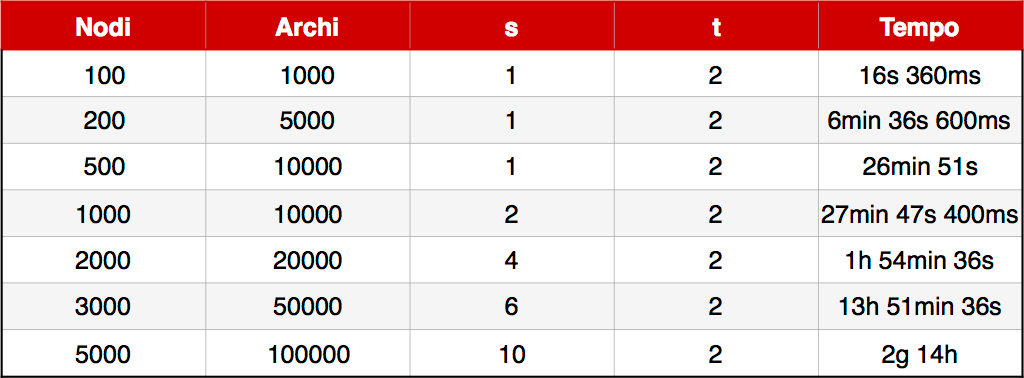
\includegraphics[scale=.6]{img/z_p2.png}
	\begin{block}{Parametri}
		\begin{itemize}
			\item $B = 20$
			\item $\beta = 0.4$
			\item $\epsilon = 0.1$
		\end{itemize}
	\end{block}
}
\subsection{Test al variare dei parametri}
\frame{
	\frametitle{Accuratezza e Razionalità}
	\begin{block}{Accuratezza $\epsilon$}
		\begin{itemize}
			\item $\epsilon \in [10^{-1},\,10^{-4}]$
			\item Running time invariato fino a $10^{-3}$
		\end{itemize}
	\end{block}
	\begin{block}{$\mu$, campo magnetico e razionalità}
		\begin{itemize}
			\item $\mu \in [1,\,0.75]$
			\item $B \in [20,\, 0.8]$
			\item $\beta \in [0.4,\,0.10]$
		\end{itemize}
	\end{block}
}
\frame{
	\frametitle{Accuratezza e Razionalità (2)}
	\centering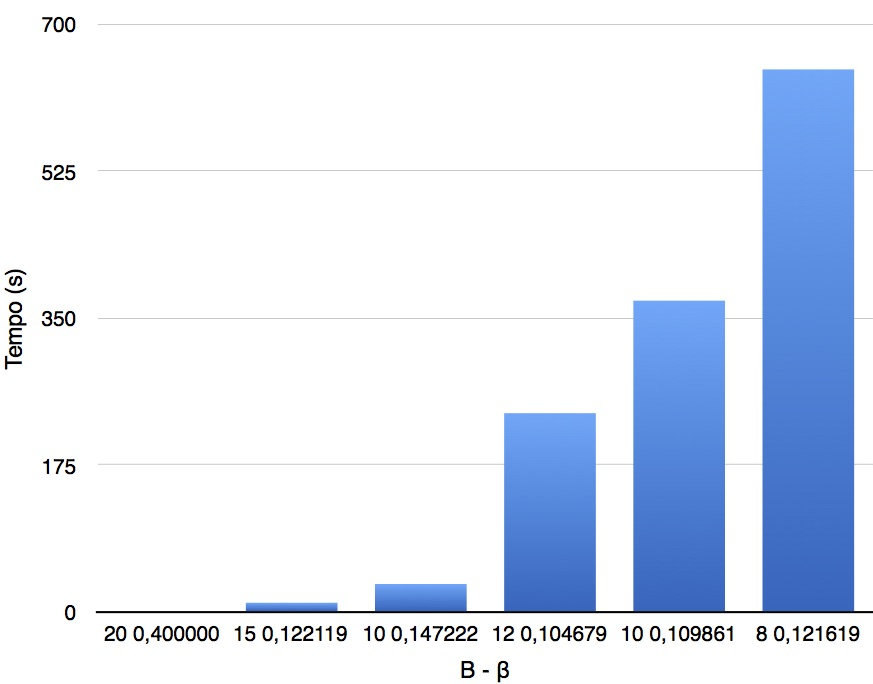
\includegraphics[scale=.2]{img/charts/Bbeta8_20.jpg}
	\begin{block}{}
		Tempo proporzionale al decrescere di campo esterno e razionalità
	\end{block}
}
\subsection{Mean Magnetic Moment}
\frame{
	\frametitle{Test di magnetizzazione}
%	\centering\textbf{\textit{Partition}}
%	\begin{table}[]
%		\centering
%		\begin{tabular}{|c|c|c|c|c|c|c|c|}
%			\hline
%			Nodi & Archi & s & t & Tempo\\ \hline
%			10& 50& 62245& 2& 14h 20m 16s\\ \hline
%		\end{tabular}
%	\end{table}
%	\centering\textbf{\textit{Partition2}}
%	\begin{table}[]
%		\centering
%		\begin{tabular}{|c|c|c|c|c|c|c|c|}
%			\hline
%			Nodi & Archi & s & t & Tempo\\ \hline
%			10& 50& 5950& 2& 3min 48s\\ \hline
%			20& 100& 13218& 2& 6min 31s\\ \hline
%			40& 250& 27754& 2& 12min 46s\\ \hline
%			100& 1000& 71361& 2& 34min 15s\\ \hline
%			500& 5000& 362075& 2& 3h 24min 17s\\ \hline
%		\end{tabular}
%	\end{table}
\centering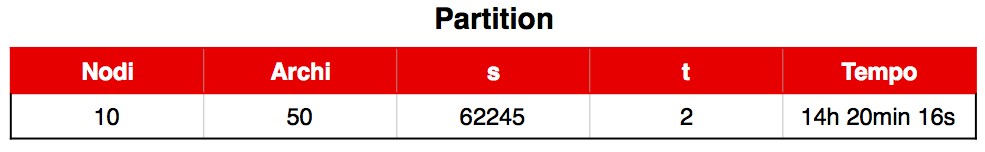
\includegraphics[scale=.3]{img/mmm_rin.png}
\vspace{20pt}
\centering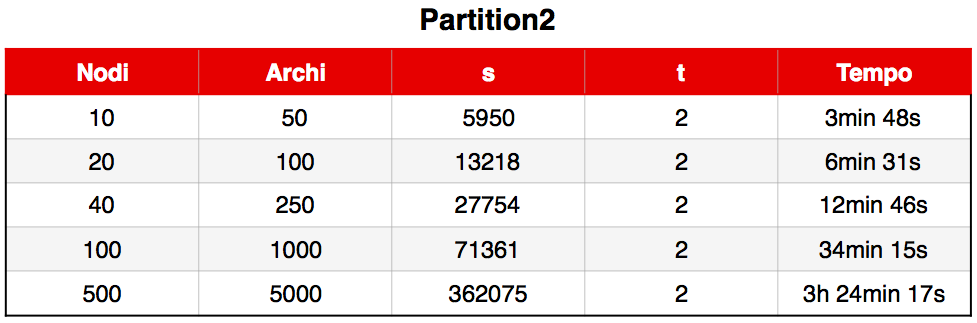
\includegraphics[scale=.3]{img/mmm_p2.png}
}
\subsection{Dataset reali}
\frame{
	\frametitle{Gnutella}
	\begin{block}{Descrizione}
		\begin{itemize}
			\item Sequenza di 9 \textit{snapshots} della rete di condivisione file \textit{peer-to-peer} Gnutella a partire da Agosto 2002
			\item Nodi: \textit{host} nella topologia della rete (6301)
			\item Archi: connessioni tra gli \textit{host} (20777)
		\end{itemize}
	\end{block}
	\begin{block}{Tempo}
		Partition function Z calcolata in circa 16 ore
	\end{block}
}
\frame{
	\frametitle{Facebook}
	\begin{block}{Descrizione}
		\begin{itemize}
			\item \textit{Snapshot} di un sottografo della rete di amicizie di Facebook
			\item Nodi: utenti della sottorete (4039)
			\item Archi: relazioni di amicizia tra utenti (88234)
		\end{itemize}
	\end{block}
	\begin{block}{Tempo}
		Partition function Z calcolata in circa 7 giorni
	\end{block}
}
%%%%%%%%%%%%%%%%%%%%%%%%%%%%%%%%%%%%%%%%%%%%%%%%%%%%%%%%%%%%%%%%%%%%%%%%%%%%
\section{Conclusioni}
\frame{
	\frametitle{Conclusioni e sviluppi futuri}
	\begin{block}{}
		\begin{itemize}
			\item Notevoli miglioramenti apportati all'algoritmo \textit{Partition}
			\item Running time ragionevoli
			\item Possibilità di testare grandi dataset
		\end{itemize}
	\end{block}
	\pause
	\begin{block}{Sviluppi futuri}
			\begin{itemize}
				\item Parallelizzare la simulazione della catena di Markov
				\item Migliorare il calcolo del \textit{mean magnetic moment}
			\end{itemize}
	\end{block}
}

\section{}
\begin{frame}{Grazie per l'attenzione}
	\begin{figure}
		\centering
		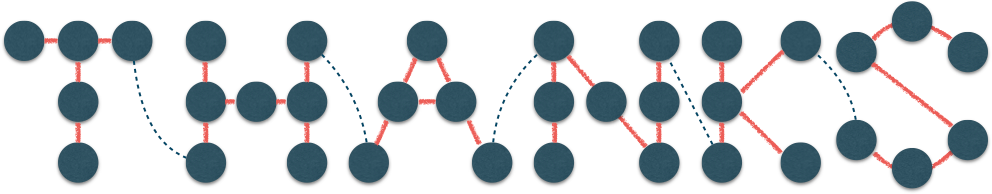
\includegraphics[scale=0.3]{img/thanks.png}
	\end{figure}
	%	\centering\animategraphics[height=2in,autoplay,controls]{12}{img/gif/ty_}{0}{56}
\end{frame}

\end{document}